% Exemple d'utilisation de la classe roadef2018 pour le congr�s ROADEF 2018 (http://roadef2018.labsticc.fr)

\documentclass{roadef}

\begin{document}


% Le titre du papier
\title{Maintenance planning on french military aircraft operations}

% Le titre court
\def\shorttitle{Titre court}

% Les auteurs et leur num�ro d'affiliation
\author{Franco Peschiera\inst{1}, Alain Ha�t\inst{1}, Olga Batta�a\inst{1} }


% Les affiliations (par ordre croissant des num�ros d'affiliation) s�par�es par \and
\institute{
ISAE... \\
\email{\{franco.peschiera\}@isae-supaero.fr}
}


% Cr�ation de la page de titre
\maketitle
\thispagestyle{empty}

% Les mots-cl�s
\keywords{optimisation, planification, militaire, maintenance}


\section{Introduction}

The Flight and Maintenance Planning is a very well known and studied problem in the aviation industry. It

...

Military Flight and Maintenance Planning...



\section{MFMP}

    \subsection{Tasks}
    \label{def:task}

    There is a set of (XXX) tasks to do in a given planning horizon divided into (XXX) periods of the same length. Each task (XXX) has a given starting (XXX) an ending (XXX) time (the duration is measured in a certain number of periods) and needs to use a certain quantity of resources (XXX). Not all (XXX) resources can be used to accomplish any task: each task has specific specifications that a resource need to satisfy in order to be a candidate. In other words, there is a parameter (XXX) that indicates task-resource compatibility. A resource can be a candidate for more than one task.

    The assignment of a resource to a task is not made necessarily for the whole duration of the task. After a minimum amount of time (XXX), a resource can be liberated and exchanged for another one. The total number of resources being used at any given time in a specific task can never be less than the required XXX.

    \subsection{Resources}

    The resources require a recurrent maintenance to be in the correct state to accomplish such tasks correctly. These maintenances need to take place before a given amount of time (ElapsedTime XXX) has passed since the previous maintenance or before the resource has been used for a given amount of time (UsageTime XXX) since the previous maintenance, whichever happens first. A resource without the proper maintenance cannot be used to satisfy tasks and is consider worthless.

    Additionally, after an absolute amount of time and/or usage, the resource becomes obsolete. There is no way to reverse this process.

    Each resources starts the planning period with a specific status given by:

    \begin{itemize}
        \item UsageTime.
        \item ElapsedTime.
        \item UsageTimeAbs.
        \item ElapseTimeAbs.
        \item LastMaintenanceType.
    \end{itemize}

    Finally, resources are organized into families or groups. Each resource inside in a family or group shares the same types of maintenances and, usually, the same kind of tasks, among other information.

    \paragraph{Resource's states}
    \label{def:res-state}

    The following are the possible states for a resource in any given time:

    \begin{itemize}
        \item Assigned to a task (see \ref{def:task}).
        \item Under maintenance (see \ref{def:maint}).
        \item Under storage (see \ref{def:sto}).
        \item Waiting maintenance.
        \item Obsolete.
        \item Available (none of the above).
    \end{itemize}

    \subsection{Maintenances}
    \label{def:maint}

    These maintenances take an amount of time equal to (XXX) periods and cannot be interrupted. The state of the resource after the maintenance period is of "as good as new" in terms of the two indicators that decide the maintenance (ElapsedTime XXX and UsageTime XXX).
    
    In other words: after a given maintenance XXX, a resource resets its ElapsedTime and UsageTime back to 0, so it can continue being assigned to tasks.

    The number of resources under maintenance in any given period is limited to a maximum capacity (XXX) depending on each period.

    Not all maintenances are the same for any given resource. Each resources follows a sequence of maintenances. In other words, the second maintenance of a given resource is different in nature from the first maintenance for that same resource. Examples of differences on consecutive maintenances are the duration it takes or whether it restores storage capacity (see \ref{def:sto}).

    \subsection{Storage}
    \label{def:sto}

    We have already explained that even if a resource is not being used, it still needs to have a maintenance after a given amount of time (ElapsedTime). In order to avoid this problem, the resource can be put into a "storage" state.

    A resource in this states has to be kept for a minimum time (XXX). While in this state it cannot receive maintenance or be assigned any task.

    \subsection{Objectives}
    
    The are multiple objectives that need to be taken into account:

    \begin{enumerate}
        \item Minimize the maximum number of resources under maintenance in any given period.
        \item Maximize the minimum number of resources available (see \ref{def:res-state}) in any given period.
    \end{enumerate}

    Every resource has the capacity to be stored. This capacity (measured in number of periods XXX) is expended every time the resource is stored. In order for a resource to recover storage capacity, it needs to received a specific maintenance.

    % \begin{figure}[!ht]
    %     \begin{center}
    %         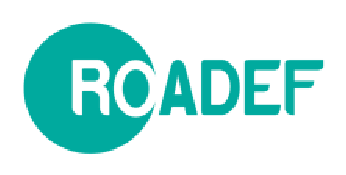
\includegraphics[height=2cm,clip=true]{roadef_logo.eps}
    %         \caption[Fig]{Logo de la ROADEF}
    %         \label{logoRoadef}
    %     \end{center}
    % \end{figure}

    % \begin{equation}
    % E=MC^2\label{emc}
    % \end{equation}

    % \begin{theoreme}
    %   Un exemple de th�or�me. Les environnements suivants sont �galement disponibles : remarque, propri�t�, corollaire, d�finition, notation, proposition, exemple, preuve.
    % \end{theoreme}

    % \subsection{Tableau}

    % Le titre du tableau devra �tre positionn� sous le tableau (par exemple Tableau \ref{tableau}).

    % \begin{table}[!ht]
    %     \begin{center}
    %         \begin{tabular}{lrr}
    %             \hline
    %             & \multicolumn{1}{c}{Colonne 1} & \multicolumn{1}{c}{Colonne 2}\\
    %             \hline
    %             Ligne 1 & L1C1 & L1C2\\
    %             Ligne 2 & L2C1 & L2C2\\
    %             \hline
    %         \end{tabular}
    %         \caption{Exemple de tableau}
    %     \label{tableau}
    %     \end{center}
    % \end{table}

    % \subsection{Liste}

    % Voici une liste :

    % \begin{itemize}
    % \item remarque
    % \item propri�t�
    % \end{itemize}

\section{Model}



    \begin{equation}
    E=MC^2\label{emc}
    \end{equation}





\section{Conclusions et perspectives}




% La bibliographie

\bibliographystyle{plain}

% Version "on-line" de la bibliographie, mais il est
% �galement possible d'utiliser un fichier ".bib" et d'utiliser BibTeX


\begin{thebibliography}{2}
\bibitem{toth02}
Paolo Toth and Daniele Vigo.
\newblock \emph{The Vehicle Routing Problem}.
\newblock Monographs on Discrete Mathematics and Applications. Society for Industrial and Applied Mathematics, 2002.
\bibitem{kirkpatrick83}
Scott Kirkpatrick, C~Daniel Gelatt, and Mario~P Vecchi.
\newblock Optimization by simmulated annealing.
\newblock \emph{science}, 220\penalty0 (4598):\penalty0 671--680, 1983.


\end{thebibliography}


\end{document}
